% TODO
% Thème pour listings
% Transitions entre les diapos


\section{Tests et analyse du code}
% Tests unitaires pour assurer la non régression
% Tests de performances pour mesurer les capacités du programme

% ---

% Remplacer par diapo de titre ?
  %\begin{frame}{Tests}{Objectifs}
  %  \begin{itemize}
  %  \item {
  %    S'assurer du bon fonctionnement de l'application reprise
  %  }
  %  \item {
  %    Vérfier que les modifications apportées au projet sont
  %    fonctionnelles
  %  }
  %  \end{itemize}
  %\end{frame}

% ---

  \begin{frame}{Tests}{Mise en place}
    Intégration dans le système de compilation:
    \begin{itemize}
      \item Un exécutable par test, compilé avec le reste du programme
        % Permet de facilement tester une seule fonctionnalité
      \item Lancement à partir du système de compilation (module CTest
        de CMake)
        % Facilité d'utilisation pour le développeur et pour un logiciel
        % d'Intégration Continue afin de lancer les tests
        % automatiquement. CTest permet de récolter des statistiques sur
        % les tests (programes de dashboard)
    \end{itemize}
  \end{frame}

% ---
  
  \begin{frame}[fragile]{Tests}{Fonctionnement}
    \textbf{Mocking}: remplacer certaines parties du programme par des
    faux afin de faciliter le test d'une fonctionnalité.
    % Dans note projet:
    \begin{itemize}
      \item Remplacer la définition d'une classe ou d'une fonction par
        un faux pour contrôler son comportement
        % Utilisé dans le projet pour "désactiver" certaines classes
        % dans le but de simplifier la construction des tests. Par
        % exemple la classe Shader inutile aux tests, ou désactiver les
        % appels OpenGL car pas de contexte
      \item Rediriger un appel de fonction pour l'effacer ou récupérer
        ses arguments grâce au préprocesseur
        \begin{lstlisting}[language=C++, basicstyle=\small]
#define glActiveTexture         (void)sizeof
// ...
#define glBufferData(t,size,buff,m) test(buff, size)
        \end{lstlisting}
    \end{itemize}
  \end{frame}

% ---

  %\begin{frame}[fragile]{Tests}{Mocking}
  %  \begin{itemize}
  %    \item Effacer un appel:
  %      \begin{lstlisting}[language=c++]
  %// Sans valeur de retour
  %#define glActiveTexture         (void)sizeof
  %// Avec valeur de retour
  %#define glCreateShader          0;(void)sizeof
  %      \end{lstlisting}
  %    \item Redirection:
  %      % Avec masquage de certains paramètres.
  %      \begin{lstlisting}[language=c++]
  %void test_update_buffer(void *buffer, size_t size);
  %// ...
  %#define glBufferData(type, size, buffer, mode) test_update_buffer(buffer, size)
  %      \end{lstlisting}
  %  \end{itemize}
  %\end{frame}

% ---

  \begin{frame}{Tests}{Exemple de test unitaire}
    \texttt{Triangulator::SplitHeuristic}:
    % Test en boite blanche: partie de l'implémentation désactivée
    % (culling) pour tester la décision de couper ou non
    % Repose sur la connaissance de l'implémentation du test. Les
    % scénarios créés sont conçus en connaissant à l'avance le résultat
    % attendu.
    \begin{itemize}
      \item Entrées: un triangle du maillage
      \item Sorties: Le status du triangle:
        \begin{itemize}
          \item Masqué
          \item A découper
          \item Feuille
        \end{itemize}
    \end{itemize}
  \end{frame}

% --- 

  \begin{frame}{Tests}{Tests de performance}
    Tests de performance de la génération de la carte de hauteur pour
    des résolutions allant de $2^6\times2^6 (64\times64)$ à
    $2^{11}\times2^{11} (2048\times2048)$
    \begin{figure}[!ht]
      \centering
      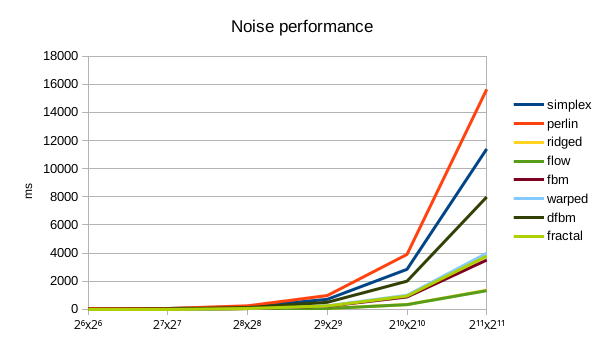
\includegraphics[width=10cm]{img/bench_i53570_fixed.png}
      \caption{Temps de génération en fonction de la complexité de la
      planète (Intel Core I5 3570)}
      \label{fig:bench}
    \end{figure}
    % Valeurs numériques données par le programme de test et importées
    % dans un tableur
  \end{frame}

% ---

  \begin{frame}{Tests}{Analyse statique}
    Objectifs:
    \begin{itemize}
      \item Améliorer la lisibilité:
        Utiliser \texttt{auto} pour ne pas répéter le type
        % Et donc la maintenabilité du code pour éviter les erreurs
      \item Moderniser le code:
        Utiliser \texttt{nullptr} au lieu de \texttt{NULL} ou de
        \texttt{0}
        % Exploiter au maximum les avantages du standard C++ utilisé
      \item Améliorer les performances
        Utiliser \texttt{emplace\_back} dans les conteneurs de la STL au
        lieu de \texttt{push\_back}.
        % Un seul constructeur au lieu d'une constructeur + copie ou
        % déplacement
    \end{itemize}
    Analyseurs utilisés:
    \begin{itemize}
      \item Clang / GCC (\texttt{-Wall -pedantic})
      \item clang-tidy
      \item cppcheck
    \end{itemize}
    Avantages:
    \begin{itemize}
      \item Intégration dans CMake
      \item Facilement configurables
      \item Correcteur automatique de clang-tidy
    \end{itemize}
  \end{frame}

% ---

\begin{frame}[fragile]{Bugs corrigés}{}
\begin{itemize}
    \item 
    Il y avait un dépassement de tableau dans le GPU(Shaders/patch.glsl l 35) lorsque la récursion s'arrêtait à l'icosaèdre (ie: lorsque la planète était trés éloignée):
\begin{lstlisting}[language=c++]
float low = distanceLUT[lev-1];
\end{lstlisting}
    \item
    La fonction SplitHeuristic désactive la vérification du frustum culling pour les futurs niveaux lorsque un triangle est totalement inclue. La fonction alternait anormalement entre ce mode "frustum culling", et le mode subdivision direct, engendrant des vérifications inutiles.
    
\end{itemize}


        
  \end{frame}
% ---
